% Measurement properties of the four geometric features, assessed before the outcome was used
% (user, 2026-10-31). COSMIN taxonomy for reliability and construct validity, QIBA terminology for
% technical performance; audit fixes from reports/Feature validity section literature audit.md.
% Main text kept short for a first read; detail for reproducing the work is in
% appendix/A_feature_validity_details.tex (sec:app-validity).
% Results go in results/01_feature_validity.tex. Literature behind the hypotheses:
% reports/Coronary geometry known correlates.md and research_notes/Coronary geometry known correlates/.
% Implementation: CGPS_data/hypertension_tortuosity.py (hypotheses, curvature); taper in
% tortuosity/taper.py.
% Not written yet: the phantom benchmark.
% Repeatability and stability are not assessed (user, 2026-10-31): no repeated scans at a short
% interval; the limitation is in discussion/feature_validity_limitations.tex.
% Figure: methodology/feature_validity_schematic.py (synthetic curves, no patient data).
% Medis is deliberately not part of this section (user, 2026-10-31); the tracer-Medis comparison
% is in methodology/01b_medis_reference.tex (sec:method-medis).
% [..] and \clarify{} mark information that is not yet available; nothing there is to be guessed.
% Tables need \usepackage{array} (ragged-right columns).
% Red clarification notes; needs \usepackage{xcolor} in the preamble. Remove before submission.
\providecommand{\clarify}[1]{\textcolor{red}{\textbf{Clarification needed:} #1}}
\section{Measurement Properties of the Geometric Features}
\label{sec:method-validity}

Whether the geometry of the coronary tree carries a risk of plaque can only be answered if the geometry is measured correctly.
If the features do not describe the arteries, a null result cannot be told apart from a failed measurement, and a positive result may come from an artifact of the extraction.
No reference standard for coronary shape exists in the Herlev--{\O}sterbro cohort, so the features were checked indirectly, without the outcome.
First, their technical accuracy was assessed on synthetic shapes with known values (Section~\ref{sec:method-validity-accuracy}).
Subsequently, one primary definition was fixed per feature, with the others kept for a sensitivity analysis (Section~\ref{sec:method-validity-definitions}).
Construct validity was then tested against hypotheses from the literature (Section~\ref{sec:method-validity-groups}), and finally the share of the variance that known risk factors explain was estimated (Section~\ref{sec:method-validity-split}).
The terms follow the COSMIN taxonomy \cite{mokkink2010cosmin} and the terminology for quantitative imaging biomarkers \cite{kessler2015qib, raunig2015qib}.
Repeatability could not be assessed, as no participant was scanned twice within a short interval; this limitation is discussed in Section~\ref{sec:disc-validity-repeatability}.
The primary definitions were fixed before any hypothesis was tested, so the hypotheses remain an independent test of them.

Figure~\ref{fig:method-validity} shows what a feature should look like.
It should differ somewhat between groups known to differ in anatomy, which suggests that it measures the arteries.
It should also vary widely within those groups, as most known risk factors are already part of SCORE2, and a feature that only repeated them could add nothing to the prediction models.

\begin{figure}[htbp]
  \centering
  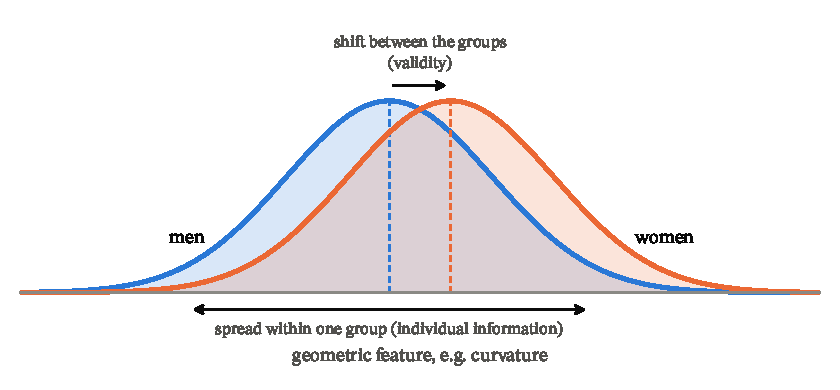
\includegraphics[width=0.75\textwidth]{methodology/feature_validity_schematic.pdf}
  \caption{Intended profile of a geometric feature: a modest difference in mean between two groups known to differ in coronary anatomy, with large variance within each group. Schematic; the curves do not show data.}
  \label{fig:method-validity}
\end{figure}

\subsection{Technical Accuracy on Synthetic Shapes}
\label{sec:method-validity-accuracy}

The first step asks whether each computation returns the right value when the right value is known.
No such value exists for a real artery, so the features were computed on synthetic shapes: arcs, helices and sine-shaped curves for curvature, tapering tubes for taper, and Y-shaped tubes for the bifurcation angle and the diameter ratios.
Two kinds of error were added.
The centerline was displaced smoothly along its length, by [..] to [..]\,mm, and the radius was perturbed, including a bias that grows as the vessel narrows.
Each definition was compared with its own value on the shape without errors, and the bias and the linearity over a range of true values were recorded \cite{raunig2015qib}.
To compare definitions with different units, the standard deviation of the error was divided by the spread of the same definition between participants in the cohort.
These shapes test how a feature is computed from a centerline, not how well the tracer finds the centerline in a scan.
The full specification is given in Appendix~\ref{sec:app-validity}.

\subsection{Definitional Choices}
\label{sec:method-validity-definitions}

Most features summarize a profile along the vessel, and the summary can be taken in several ways.
Curvature, for example, depends on the chord over which the turning angles are measured and on whether they are averaged, counted as bends or reduced to the largest turn.
A primary definition was therefore fixed for each feature, and the others were kept as alternatives (Table~\ref{tab:method-validity-definitions}).

\begin{table}[htbp]
  \centering
  \caption{Primary definition of each feature and the alternatives used in the sensitivity analysis.}
  \label{tab:method-validity-definitions}
  \small
  \begin{tabular}{>{\raggedright\arraybackslash}p{1.9cm}>{\raggedright\arraybackslash}p{4.6cm}>{\raggedright\arraybackslash}p{4.6cm}}
    \toprule
    Feature & Primary definition & Alternatives \\
    \midrule
    Curvature & mean turning angle per millimeter at a chord of 5\,mm (Section~\ref{sec:method-curvature}) & chords of 2.5 and 10\,mm; count of bends \cite{bullitt2003tortuosity}; 90th percentile; largest turning angle \\
    \addlinespace
    Taper & slope of the logarithm of the area-equivalent radius, fitted with the Theil--Sen estimator, excluding the first 3\,mm and side-branch origins & ratio of the radii at the two ends; radius from the distance transform; no exclusions \\
    \addlinespace
    Diameter ratios & area-equivalent diameters [..]\,mm from the carina \clarify{sampling distance.} & other distances; minimum diameter \\
    \addlinespace
    LM bifurcation angle & angle between the LAD and LCx directions fitted over the first [..]\,mm \clarify{fitting length.} & fitting over 5 and 10\,mm; ramus intermedius treated as the LCx or excluded \\
    \bottomrule
  \end{tabular}
\end{table}

The primary definitions were chosen on technical accuracy and the literature.
For curvature, the literature favored the mean absolute curvature, which tracked low wall shear stress best in 127 coronary CT scans, while the arc-to-chord ratio did not \cite{kashyap2022tortuosity}.
The hypotheses of step 3 were never used to choose, as the same data would then both select and test a definition.
Even the angle, which looks simple, depends on how far along each branch its direction is fitted and on whether a ramus intermedius is taken for the LCx.

\label{sec:method-validity-sensitivity}
In the sensitivity analysis, every hypothesis was recomputed for each alternative and reported without changing the primary definition.
Definitions can disagree: tortuosity counted as bends has been linked to less coronary disease \cite{li2011tortuosity}, and tortuosity measured as a mean turning angle to slightly more \cite{telloayala2026tortuosity}.

\subsection{Construct Validity}
\label{sec:method-validity-groups}

The third step asks whether each feature behaves as the literature says the anatomy behaves, which is called construct validity \cite{mokkink2010cosmin}.
It was tested with hypotheses formulated before the data were seen \cite{cronbach1955construct, prinsen2018cosmin}, listed in Table~\ref{tab:method-validity}.
Known-groups hypotheses state how much a feature differs between groups, such as women and men.
An internal-relationship hypothesis states a value that follows from a known law, here the scaling of diameters at a bifurcation.
Discriminant hypotheses state that a feature is unrelated to variables with no known link to vessel shape; an association with one of these would point to a shared error, such as image quality.

Each hypothesis states a size as well as a direction \cite{terwee2007quality, prinsen2018cosmin}.
It was confirmed when the estimate fell within its expected range, expressed in standard deviations of the feature or, for the angle, in degrees.
Statistical significance was not used, as with about 1,200 participants even a trivial difference is significant.
A hypothesis of no difference was confirmed only when the 90\% confidence interval lay within $\pm 0.2$ standard deviations, as an interval that merely includes zero shows an absence of evidence, not of an effect \cite{lakens2017equivalence}.
All estimates were adjusted for age.
Each hypothesis states whether its estimate is also adjusted for body size, matching the study it rests on, as adjusting a sex difference for body size answers a different question \cite{schisterman2009overadjustment}.
\clarify{confirmation of the expected ranges before the data are opened.}

\begin{table}[htbp]
  \centering
  \caption{Hypotheses for construct validity. Type: K, known-groups; I, internal relationship; D, discriminant. SD is the standard deviation of the feature; hypotheses of no difference are confirmed when the 90\% confidence interval lies within $\pm 0.2$ SD. Evidence is the author's judgement (Section~\ref{sec:method-validity-evidence}).}
  \label{tab:method-validity}
  \footnotesize
  \setlength{\tabcolsep}{4pt}
  \begin{tabular}{>{\raggedright\arraybackslash}p{1.4cm}>{\raggedright\arraybackslash}p{1.9cm}>{\raggedright\arraybackslash}p{0.6cm}>{\raggedright\arraybackslash}p{3.3cm}>{\raggedright\arraybackslash}p{2.5cm}>{\raggedright\arraybackslash}p{1.3cm}}
    \toprule
    Feature & Hypothesis & Type & Expected value & Variable & Evidence \\
    \midrule
    Curvature & women vs men & K & women higher by 0.2 to 1.0 SD, without adjustment for body size \cite{li2011tortuosity, li2022tortuosity, telloayala2026tortuosity, sharfo2024tortuosity, gharleghi2024leftmain} & \texttt{male} & strong \\
     & hypertension & K & higher with hypertension, by less than the difference between the sexes \cite{li2011tortuosity, li2022tortuosity, telloayala2026tortuosity, sharfo2024tortuosity} & \texttt{med\_\allowbreak antihypertensive\_\allowbreak any} & moderate \\
     & LDL, smoking, family history & D & within $\pm 0.2$ SD \cite{groves2009tortuosity} & \texttt{ldl}, \texttt{hist\_\allowbreak smoking\_\allowbreak current}, \texttt{demo\_\allowbreak hist\_\allowbreak family\_\allowbreak cvd} & weak \\
    \addlinespace
    Taper & mean diameter, men vs women & K & 5 to 30\% larger in men \cite{dodge1992diameter} & \texttt{male} & strong \\
     & fractional taper, sex and body size & K & within $\pm 0.2$ SD & \texttt{male}, \texttt{clin\_\allowbreak bsa} & weak \\
     & LAD vs RCA & K & LAD steeper by at least 0.2 SD, within participant \clarify{citation; only a secondary source (Zubaid et al.\ 2002) was found.} & artery & weak \\
    \addlinespace
    LM bifurcation angle & men vs women & K & 5 to 15$^{\circ}$ wider in men, adjusted for height \cite{medranogracia2016atlas} & \texttt{male}, \texttt{clin\_\allowbreak height} & weak \\
     & ramus intermedius & K & 7 to 21$^{\circ}$ wider with a ramus \cite{medranogracia2016atlas} & from the tree \clarify{whether \texttt{ct\_\allowbreak cag\_\allowbreak im\_\allowbreak eval} marks a present ramus.} & weak \\
    \addlinespace
    Diameter ratios & left vs right dominance & K & LCx larger relative to the LM by at least 0.2 SD in left dominance \cite{dodge1992diameter} & \texttt{ct\_\allowbreak cag\_\allowbreak dominance} & weak \\
     & women vs men & K & within $\pm 0.2$ SD \cite{medranogracia2016atlas} & \texttt{male} & weak \\
     & scaling law & I & cohort median of the Finet ratio 0.60 to 0.72 \cite{finet2008fractal, huo2012scaling, taylor2024murray, medranogracia2016atlas} & none & moderate \\
    \bottomrule
  \end{tabular}
\end{table}

\label{sec:method-validity-evidence}
The hypotheses do not rest on equally firm evidence, so each was graded strong, moderate or weak according to how consistently the studies found the association; the grades and their limits are detailed in Appendix~\ref{sec:app-validity}.
The higher curvature in women illustrates a strong grade.
Six studies, using different imaging and different definitions of tortuosity, all found it, and none found the opposite (Table~\ref{tab:method-validity-sex}).
Even so, nearly all of them studied patients referred with chest pain, and only a preprint of 127 scans measured curvature as in this thesis \cite{gharleghi2024leftmain}.
The same difference could also arise from the measurement itself, as narrower arteries give noisier centerlines and noise adds apparent curvature, so a confirmation was read together with the result at the longer chord, where noise matters less.

\subsection{Variance Explained by Known Risk Factors}
\label{sec:method-validity-split}

The last step asks how much of the variation in a feature is already explained by the risk factors in the models.
For each feature, $R^2$ was computed from a linear regression on the covariates of the base model, the refitted SCORE2 factors.
A high $R^2$ would make the feature largely a repeat of these covariates, with little left for the likelihood-ratio test of the geometry block to detect.
The remaining share, $1 - R^2$, is the room left for geometry.
Without a repeated measurement, this share cannot be divided into anatomy that differs between people, which could relate to plaque, and measurement error, which could not (Section~\ref{sec:disc-validity-repeatability}).

\subsection{Decision Rules}
\label{sec:method-validity-reading}

A feature was kept unchanged when all of its hypotheses graded strong were confirmed.
Features without a strong hypothesis were kept, and their construct validity was reported descriptively; the share of confirmed hypotheses was reported for every feature rather than used as a cut-off.
A feature that failed was checked for errors in its extraction.
If its primary definition still failed, it was replaced by the alternative with the smallest scale-free error in Section~\ref{sec:method-validity-accuracy}, never by the one that best fitted the hypotheses.
\clarify{what is done when no alternative passes either: dropped, or kept and reported with its failed hypotheses.}
All definitions, settings and expected ranges were fixed on [date], before the outcome was linked to the geometry.
